%#!ptex2pdf -l -u -ot '--synctex=1' -od '-z 3' readme-kddbook
% #!ptex2pdf -l -u -s -ot '--synctex=1' -od '-z 3' readme-kddbook && ptex2pdf -l -u -s -ot '--synctex=1' -od '-z 3' readme-kddbook && upmendex -r -c -g -s kddbook.ist -- readme-kddbook && ptex2pdf -l -u -ot '--synctex=1' -od '-z 3' readme-kddbook
\documentclass[dvipdfmx,%%<= 特別な事情がないかぎり、有効にしてください。
  tombo,%%<= トンボを付けて、ご入稿ください。
  paper=b5,%default: a5; available: a5, b5
]{kddbook}

%% 必要に応じて、各種パッケージ
%% 下記で読み込んでいるパッケージたちは、一例です。
%% tcolorbox パッケージなど利用しない場合、
%% 下記の \newtcolorbox による設定などを削除してください。
\usepackage{graphicx}
% \graphicspath{{./},{images/},{figs/}}
\usepackage[table]{xcolor}
% \usepackage{plistings}
\usepackage{tcolorbox}
\tcbuselibrary{skins,breakable}
\usepackage{amssymb}
\usepackage{amsthm}
\usepackage{bm}
\usepackage{enumerate}

\newtcolorbox{kddframed}{%
  empty, 
  before skip=\baselineskip,
  after skip=\baselineskip,
  boxsep=3mm, boxrule=0mm, 
  top=0mm, bottom=0mm, left=0mm, right=0mm, 
  breakable, pad at break=.25zw,
  enlargepage flexible=.5zw,
  borderline={0.1mm}{0mm}{black}, arc=0mm, 
}

\newtcolorbox{kddshaded}{%
  enhanced, frame empty, 
  before skip=\baselineskip,
  after skip=\baselineskip,
  boxsep=3mm, boxrule=0mm, 
  top=0mm, bottom=0mm, left=0mm, right=0mm, 
  breakable, pad at break=.25zw, 
  colback=black!15, arc=0mm,
}

\newtcolorbox{kddcolumn}[1][]{%
  empty, 
  before skip=\baselineskip,
  after skip=\baselineskip,
  boxsep=3mm, boxrule=0mm, 
  left skip=10mm,
  top=0mm, bottom=0mm, left=-3mm, right=-3mm, 
  breakable, pad at break=.25zw,
  enlargepage flexible=.5zw,
  fontupper={\setlength{\parindent}{1zw}},
  borderline north={0.2mm}{0mm}{black}, 
  borderline south={0.2mm}{0mm}{black}, 
  coltitle=black, fonttitle={\bfseries}, 
  before upper={\noindent\tcbtitle\par},
  detach title, title={#1},
}


\title{初めてのディジタル信号処理}
\author{田中賢一}
\date{2021/10/31}

\begin{document}
\frontmatter
%\maketitle


\chapter{まえがき}

信号処理とは,電気回路などの知識をベースとして,音声・画像処理のために大切な知識として位置づけられている.その知識を持ってフィルタの設計などを効率よく行うことができる.

ところで,信号処理という枠組みの科目自体は,電子系もしくは情報系ではほぼ必須アイテムのひとつとされて久しい.また,大学生向けのテキストとしては従来良書と分類されるものも非常に多い.しかしながら,昨今,大学における入試形態の多様化や,カリキュラムの多様性も相まって,従来のテキストで講義を行うための数学的前提条件が十分に整っていない状態であることが非常に多いという声を多く聞くようになってきた.

このことから,本書では,従来の信号処理のテキストにおける内容をできるだけ平易化することだけでなく,必要と思われる数学的なアプローチも随所に記載をして,理解しやすさに重きをおいた.したがって,高等学校で数学III程度の内容がある程度理解できるようであれば,十分に読み進められるように配慮していており,その補完として第2章において数学的な扱いをあえて示している.

また,ディジタルフィルタだけでなく,実用上組み合わせて使用することから知っておくほうがよいと考えるアナログフィルタすなわち電気回路で構成される高域フィルタ,低域フィルタなどについても説明した.最終章では画像のディジタル処理の一部についても紹介し,昨今,多く出回っているアプリケーションプログラムにおける処理のあり方についても述べた.これらを通じて,信号処理をすることにより,ユーザにとって都合の良い信号を抽出し,パターン認識や各種メディア信号処理をすることが理解されれば幸いである.

もちろん,本書で学習したならば,従来より存在する良書により,エンジニアとして必要なさらに高度な知識や教養を身につけて,社会に羽ばたいてほしいと願っている.

さて,授業を行うにあたっては教員の裁量を最優先することは大切なことと承知しているが,もし,本書を用いて90分授業を15週かけて実施する場合には,第\ref{chapter:2}章,第\ref{chapter:ch-2}章,第\ref{chapter:fft}章を2回の授業に分割して授業を行うことを想定している.特に第2章の扱いは受講者の習熟度にあわせて適宜調整されるものと考えている.

著者の浅学非才を顧みず,伝統的な良書への橋渡しのつもりで執筆したが,自分で課題を見つけて回路を実装したり,アプリケーションプログラムを作成したり,さらに深い学びを得るための準備として参考になれば幸いである.
\begin{flushright}
2022年2月\\田中 賢一
\end{flushright}



\tableofcontents

\mainmatter

%第1章
\input{text/text-intro-1}
%第2章 演習問題付き
\input{text/text-math}
%第3章  演習問題付き
\input{text/text-intro}
%第4章 演習問題付き
\input{text/text-signal}
%第5章 演習問題付き
\input{text/text-z-transform}
%第6章 演習問題付き
\input{text/text-z-2}
%第7章 演習問題付き
\input{text/text-sampling}
%第8章 演習問題付き
\input{text/text-a-filter}
%第9章 演習問題付き
\input{text/text-dft}
%
\begin{lead}

����ꂪ���ɂ��鉹���͈�ʓI�Ɏ�X�̎��g���������琬�藧���Ă���D���̎�X�̎��g���������ǂ̂悤�ɐ��藧���Ă��邩��m�邽�߂ɁC�t�[���G�ϊ���p���ĉ�͂�����@���K������D�܂��C�����M������{���g���̐����{�̎��g���������݂���Ƃ����l���̂��ƁC���`�V�X�e���̉�͂ɂ‚��Ă��K������D

\end{lead}

%\vfill

%\begin{koumoku}
%�A�i���O�t�B���^\\
%�d�C��H\\
%�𗬓d�C��H\\
%���g������\\
%���t�B���^\\
%����t�B���^\\
%�ш�t�B���^
%\end{koumoku}

%\clearpage

\chapter{�t�[���G�����E�t�[���G�ϊ�}

\label{chapter:f}

\section{�t�[���G����}

�����ł́C��������I�ȐM��$f(t)=f(t+nT)$($n$�͔C�ӂ̐���)���l����D���̂Ƃ��C$f(t)$����{�p���g��$\omega_0$�̐����{�ɂ��O�p�֐�����Ȃ鋉���ŕ\���ƁC�����̂悤�ɕ\�����D
\begin{equation}
f(t)=\frac{a_o}{2}+\sum_{n=1}^{\infty}(a_n \cos n\omega_0 t + b_n \sin n\omega_0 t)
\label{eqn:fourier-kyusu}
\end{equation}
���̎�(\ref{eqn:fourier-kyusu})�����t�[���G�����ƌĂ�ł���D�����Ŋ�{�p���g��$\omega_0$�i�P�ʂ�[rad/s]�j�́C
\begin{equation}
\omega_0=\frac{2\pi}{T}
\label{eqn:fourier-omega_0}
\end{equation}
�ł���D���̂��Ƃ���C��������I�ȐM��$f(t)=f(t+nT)$($n$�͔C�ӂ̐���)�́C��{���g���̐����{�Ɋւ��鐳���g��]���g�̘a�ŕ\�����Ƃ������Ƃ��ł���D

�����ŁC��(\ref{eqn:fourier-kyusu})�ɂ�����$a_0$�C$a_n$�C$b_n$�͎��t�[���G�W��\footnotemark �ƌĂ΂����̂ł���C�����ŕ\�����D

\footnotetext{���t�[���G�W�� \\ �Ƃ���ŁC��(\ref{eqn:fourier_a_n})�ɂ�����$n=0$�Ƃ����ꍇ�ɂ�$\cos n\omega_0 t=1$����ɐ������邽�߁C
\begin{eqnarray}
a_0&=&\frac{2}{T}\int^{\frac{T}{2}}_{-\frac{T}{2}}f(t) \cos n\omega_0 t dt \nonumber \\
 &=& \frac{2}{T}\int^{\frac{T}{2}}_{-\frac{T}{2}}f(t)dt \nonumber
\end{eqnarray}
�ƂȂ邱�Ƃ���C��(\ref{eqn:fourier_a_0})�ɋA������D
}

\begin{eqnarray}
a_0&=&\frac{2}{T}\int^{\frac{T}{2}}_{-\frac{T}{2}}f(t)dt \label{eqn:fourier_a_0}\\
a_n&=&\frac{2}{T}\int^{\frac{T}{2}}_{-\frac{T}{2}}f(t) \cos n\omega_0 t dt \hspace{1cm} (n=1,2,\cdots) \label{eqn:fourier_a_n} \\
b_n&=&\frac{2}{T}\int^{\frac{T}{2}}_{-\frac{T}{2}}f(t) \sin n\omega_0 t dt \hspace{1cm} (n=1,2,\cdots)
\end{eqnarray}

\subsection*{���4.1}
�}\ref{fig:kukeiha}�Ɏ�����`�g�ɂ‚��āC�t�[���G�����W�J������D




\begin{equation}
f(t)= \left \{
\begin{array}{ll}
1 & (0 \leq t < \pi) \\
0 & (\pi \leq t < 2\pi)
\end{array}
\right .
\end{equation}


\begin{figure}[h]
\begin{center}
\includegraphics[width=6cm]{fig/kukeiha.eps}
\caption{��`�g}
\label{fig:kukeiha}
\end{center}
\end{figure}

���̋�`�g�ɂ‚��āC���t�[���G�W��$a_0$�C$a_n$�C$b_n$�����ꂼ�ꋁ�߂�ƁC
\begin{eqnarray}
a_0 & = & \frac{2}{T}\int^{\frac{T}{2}}_{0} dt\nonumber \\
 & = & 1 - 0  \nonumber \\
 & = & 1
\end{eqnarray}
\begin{eqnarray}
a_n & = & \frac{2}{T}\int^{\frac{T}{2}}_{0}\cos \left( 2\pi k \frac{t}{T} \right) dt\nonumber \\
 & = & \frac{1}{\pi k} (\sin k\pi - \sin 0 ) \nonumber \\
 & = & 0
\end{eqnarray}
\begin{eqnarray}
b_n & = & \frac{2}{T}\int^{\frac{T}{2}}_{0}\sin \left( 2\pi k \frac{t}{T} \right) dt\nonumber \\
 & = & \frac{1}{\pi k} ( - \cos k\pi + \cos 0) \nonumber \\
 & = & \left \{
\begin{array}{cc}
\displaystyle \frac{2}{\pi k} & k=1,3,5,\cdots \\
0 & k=2,4,6,\cdots
\end{array}
\right .
\end{eqnarray}

\section{�t�[���G�����W�J�̕��f�\��}

��q�Ɠ��l�ɁC��������I�ȐM��$f(t)=f(t+nT)$($n$�͔C�ӂ̐���)���l����D���̂Ƃ��C$f(t)$����{�p���g��$\omega_0$�̐����{�ɂ��w���֐�����Ȃ鋉���ŕ\���D�Ƃ���ŁC$\sqrt{-1}=j$\footnotemark �Ƃ������̂Ɖ��肵�āC�I�C���[�̌����ɂ��΁C�w���֐��ƎO�p�֐��̊Ԃɂ�

\footnotetext{���f���̈��� \\ ���w�̋��ȏ��Ȃǂ̂悤�ɑ����̏ꍇ
\begin{equation}
i=\sqrt{-1}
\end{equation}
�ƕW�L���邪�C�d�C�d�q�H�w����H�w�Ȃǂ̕���ł́C$i$��d���Ƃ��Ă̕ϐ��Ƃ��ėp���邽�߁C����������邽�߂�$j$��p���邱�ƂƂ��āC
\begin{equation}
j=\sqrt{-1}
\end{equation}
�ƕW�L���銵�Ⴊ����D
}
\begin{equation}
e^{j\theta}=\cos \theta + j \sin \theta
\end{equation}
\begin{equation}
\cos \theta=\frac{e^{j\theta}+e^{-j\theta}}{2}
\end{equation}
\begin{equation}
\sin \theta=\frac{e^{j\theta}-e^{-j\theta}}{2j}
\end{equation}

�Ȃ�֌W�����邱�Ƃ��m���Ă���̂ŁC���ƁC�����̂悤�ɕ\�����D
\begin{eqnarray}
f(t)&=&\frac{a_0}{2}+\sum_{n=1}^{\infty}(a_n \cos n\omega_0 t + b_n \sin n\omega_0 t) \nonumber \\
 &=&\frac{a_0}{2}+\sum_{n=1}^{\infty}(a_n \frac{e^{jn\omega_0 t}+e^{-jn\omega_0 t}}{2} + b_n \frac{e^{jn\omega_0 t}-e^{-jn\omega_0 t}}{2j}) \nonumber \\
 &=&\frac{a_0}{2}+\sum_{n=1}^{\infty}\left ( \frac{a_n-jb_n}{2} e^{jn\omega_0 t}+\frac{a_n+jb_n}{2}e^{-jn\omega_0 t} \right ) \nonumber \\
 &=&\sum_{n=0}^{\infty}\left ( c_n e^{jn\omega_0 t}+c_{-n} e^{-jn\omega_0 t} \right ) \\
\label{eqn:fourier_c_n}
 &=&\sum_{n=-\infty}^{\infty} c_n e^{jn\omega_0 t}
\label{eqn:fourier-kyusu2}
\end{eqnarray}
���̎�(\ref{eqn:fourier-kyusu})�𕡑f�t�[���G�����ƌĂ�ł���D�����Ŋ�{�p���g��$\omega_0$�i�P�ʂ�[rad/s]�j�́C
\begin{equation}
\omega_0=\frac{2\pi}{T}
\label{eqn:fourier-omega_0}
\end{equation}
�ł���D���̂��Ƃ���C��������I�ȐM��$f(t)=f(t+nT)$($n$�͔C�ӂ̐���)�́C��{���g���̐����{�Ɋւ��鐳���g��]���g�̘a�ŕ\�����Ƃ������Ƃ��ł���D

�����ŁC��(\ref{eqn:fourier-kyusu})�ɂ�����$c_n$�͕��f�t�[���G�W��\footnotemark �ƌĂ΂����̂ł���C�����ŕ\�����D

\footnotetext{���f�t�[���G�W�� \\ �Ƃ���ŁC��(\ref{eqn:fourier_c_n})�ɂ�����$c_n$��$c_{-n}$�Ƃ̊Ԃɂ́C���f�����̊֌W�����邽�߁C��(\ref{eqn:fourier-kyusu2})�ɋA������D
}

\begin{eqnarray}
c_n&=&\frac{1}{T}\int^{\frac{T}{2}}_{-\frac{T}{2}}f(t) e^{ -jn\omega_0 t } dt \hspace{1cm} (n=0,1,2,\cdots)
\end{eqnarray}

\subsection*{���4.2}
�}\ref{fig:kukeiha2}�Ɏ�����`�g�ɂ‚��āC�t�[���G�����W�J������D




\begin{equation}
f(t)= \left \{
\begin{array}{ll}
1 & (0 \leq t < \pi) \\
0 & (\pi \leq t < 2\pi)
\end{array}
\right .
\end{equation}


\begin{figure}[h]
\begin{center}
\includegraphics[width=6cm]{fig/kukeiha.eps}
\caption{��`�g}
\label{fig:kukeiha2}
\end{center}
\end{figure}

���̋�`�g�ɂ‚��āC���t�[���G�W��$a_0$�C$a_n$�C$b_n$�����ꂼ�ꋁ�߂�ƁC
\begin{eqnarray}
c_n & = & \frac{1}{T}\int^{\frac{T}{2}}_{-\frac{T}{2}} e^{\left (-j2n \pi \frac{t}{T} \right )}dt \nonumber \\
 & = & \frac{1}{2jn\pi} \left ( e^{n \pi } - e^{-n \pi} \right )  \nonumber \\
 & = & \frac{1}{n \pi} \frac{\left ( e^{n \pi } - e^{-n \pi} \right )}{2j} \nonumber \\
 & = & \frac{\sin n \pi}{n \pi} \nonumber \\
 & = & sinc n\pi
\end{eqnarray}
\begin{eqnarray}
a_n & = & \frac{2}{T}\int^{\frac{T}{2}}_{0}\cos \left( 2\pi k \frac{t}{T} \right) dt\nonumber \\
 & = & \frac{1}{\pi k} (\sin k\pi - \sin 0 ) \nonumber \\
 & = & 0
\end{eqnarray}
\begin{eqnarray}
b_n & = & \frac{2}{T}\int^{\frac{T}{2}}_{0}\sin \left( 2\pi k \frac{t}{T} \right) dt\nonumber \\
 & = & \frac{1}{\pi k} ( - \cos k\pi + \cos 0) \nonumber \\
 & = & \left \{
\begin{array}{cc}
\displaystyle \frac{2}{\pi k} & k=1,3,5,\cdots \\
0 & k=2,4,6,\cdots
\end{array}
\right .
\end{eqnarray}

\section{�t�[���G�ϊ�}

\subsection{�t�[���G�ϊ��̒�`}

������I�ȘA���M��$f(t)$���l����D�}\ref{fig:hishuki-1}(a)�Ɏ����M���́C$t=0$�̎��ӂɃp���X��1�‘��݂��邾���ł��邱�Ƃ���C�����M���ł͂Ȃ��C������M���ł���D���̂悤�Ȕ�����M���̎��g����́C���Ȃ킿���ԗ̈�Ǝ��g���̈�Ƃ̕ϊ��͎����ɂ��s����D

\begin{equation}
X(\Omega)=\int^{\infty}_{-\infty}x(t)e^{-j\Omega t}d \Omega
\label{eqn:fourier-3}
\end{equation}
\begin{equation}
x(t)=\frac{1}{2\pi} \int^{\infty}_{-\infty}X(\Omega)e^{j\Omega t}d \Omega
\label{eqn:inv_fourier-3}
\end{equation}

�����ŁC��(\ref{eqn:fourier-3})�̓t�[���G�ϊ��ƌĂсC���ԗ̈�$x(t)$������g���̈�$X(\Omega)$�ւ̕ϊ����ł���D�܂��C��(\ref{eqn:inv_fourier-3})�͋t�t�[���G�ϊ��ƌĂсC���g���̈�$X(\Omega)$���玞�ԗ̈�$x(t)$�ւ̕ϊ����ł���D�܂��C�����Ŏ������t�[���G�ϊ��i��(\ref{eqn:fourier-3})�j�Ȃ�тɋt�t�[���G�ϊ��i��(\ref{eqn:inv_fourier-3})�j�̗����̑��̂��t�[���G�ϊ��ƌĂԂ��Ƃ�����D

\subsection*{���4.3}
�}\ref{fig:kukeiha5}�Ɏ�����`�g�ɂ‚��āC�t�[���G�����W�J������D

\begin{equation}
x(t)= \left \{
\begin{array}{ll}
1 & (-T_1 \leq t < T_1) \\
0 & (����ȊO)
\end{array}
\right .
\end{equation}

\begin{figure}[h]
\begin{center}
\includegraphics[width=6cm]{fig/kukeiha.eps}
\caption{��`�g}
\label{fig:kukeiha5}
\end{center}
\end{figure}

�y�𓚁z��(\ref{eqn:fourier-3})���\footnotemark �C

\begin{eqnarray}
X(\Omega)&=&\int^{\infty}_{-\infty}x(t)e^{-j\Omega t}d t \nonumber \\
&=&\int^{T_1}_{-T_1}e^{-j\Omega t}d t \nonumber \\
&=&-\frac{1}{j\Omega} \left ( e^{-j\Omega T_1} - e^{j\Omega T_1} \right ) \nonumber \\
&=&2T_1 \frac{e^{j\Omega T_1} - e^{-j\Omega T_1}}{2j\Omega T_1} \nonumber \\
&=&T_1 \mathrm{sinc}(\Omega T_1) 
\end{eqnarray}

\footnotetext{sinc�֐� \\ �M�������Ȃǂő����p������֐��ł���C
\begin{equation}
\mathrm{sinc}(x)=\frac{\sin x}{x}
\end{equation}
�Ə������D�Ȃ��C$x=0$�ƂȂ�ꍇ�ɂ́C
\begin{eqnarray}
\lim_{x \to 0}\mathrm{sinc}(x)&=&\lim_{x \to 0}\frac{\sin x}{x} \nonumber \\
 &=&\lim_{x \to 0}\frac{\cos x}{1} \nonumber \\
 &=& 1
\end{eqnarray}
�ƂȂ�D
}

\section*{���K���}

\subsection*{���\ref{chapter:f}.1}

�ȉ��̋tz�ϊ����C�ׂ������W�J�@�܂��͕��������W�J�@��p���ċ��߂�D

(1) $X(z)=z^2+2+2z^{-3}$

(2) $X(z)=\displaystyle \frac{1}{1-0.5z^{-1}}$

(3) $X(z)=\displaystyle \frac{2z^{-1}}{1-0.5z^{-1}} + \frac{1}{1-z^{-1}}$

(4) $X(z)=\displaystyle \frac{1}{(1-0.5z^{-1})(1-z^{-1})}$

\subsection*{���\ref{chapter:f}.2}

�ȉ��̃V�X�e���̓`�B�֐������߁C�n�[�h�E�F�A�\���������D

(1) $y(n)=x(n)+ax(n-1)+bx(n-2)$

(2) $y(n)=x(n)+ax(n-1)+by(n-2)$

(3) $y(n)=x(n)+ay(n-1)+by(n-2)$

\subsection*{���\ref{chapter:f}.3}

�ȉ��̃V�X�e���ɂ�������g�������C�`�B�֐��̋ɂ����ꂼ�ꋁ�߈��萫�𔻕ʂ���D

(1) $H(z)=1+2z^{-1}+z^{-2}$

(2) $H(z)=\displaystyle \frac{1+2z^{-1}}{2+z^{-1}}$




%第10章 演習問題付き
\input{text/text-fft}
%第11章 演習問題付き
\input{text/text-window}
%第12章 演習問題付き
\input{text/text-d-filter}
%第13章 演習問題付き
\input{text/text-digital-image-1}

\clearpage
%第13章

%\begin{lead}
%種々の信号処理は,信号処理システムにより実現される.そこで,ここでは離散時間信号を処理するシステムの考え方を導入する.ここで説明するシステムは,線形時不変システムと呼ばれるもので,非常に多く応用されている.信号値の乗算,加減算,信号値を記憶して時間シフト,の3種類の処理の組合せとして,ハードウェア,ソフトウェアのどちらでも実現可能である.

%\end{lead}

%\vfill

%\begin{koumoku}
%信号処理システム\\
%線形時不変システム\\
%3点平均\\
%\end{koumoku}


%\chapter{信号処理システム}
%\label{chapter:ch-2}



\section*{章末問題の略解}
\addtocontents{toc}{\onelineskip}\addcontentsline{toc}{section}{章末問題の略解}
\stepcounter{chapter}
\subsection*{第\ref{chapter:intro}章}

\subsubsection*{問題\ref{chapter:intro}.1}

画像の幾何学的形状の変形は,座標系に拡大・縮小・回転を加えることで実現可能である.たとえば眼だけ大きく見せるためには,眼の中心部分に原点をおき,眼が存在する領域だけ拡大できるように座標系を置き換えればよい.

\subsubsection*{問題\ref{chapter:intro}.2}

画像の尖鋭化を行う場合,輪郭となる部分が強調されるという長所があるとともに,ごま塩雑音などのような雑音も強調されるという短所がある.

画像のぼかしを行う場合,ごま塩雑音などのような雑音が低減されるという長所があるとともに,輪郭となる部分がぼけてしまうという短所がある.

\subsubsection*{問題\ref{chapter:intro}.3}

人間の可聴音は20Hz~20kHzであるとされている.その上限である20kHzの2倍以上である44.1kHzであれば,サンプリング定理により20kHzの音声信号を復元可能とされるためである.

\subsection*{第\ref{chapter:2}章}

\subsubsection*{問題\ref{chapter:2}.1}

\noindent (1) $A=1$,$\theta=\displaystyle \frac{-\pi}{3}$,
(2) $A=\sqrt{(1+\displaystyle \cos \frac{-\pi}{3})^2+\sin^2 \theta}=\displaystyle \frac{\sqrt{15}}{2}$,$\theta=\tan^{-1}\displaystyle \frac{2}{3}$,\\
(3) $A=\displaystyle \frac{\sqrt{(x^2-9)^2 + 36x^2}}{x^2+9}$,$\theta=\displaystyle \frac{6x}{(x^2-9)}$,
(4) $A=\displaystyle \sqrt{ R^2+ \left( \omega L - \frac{1}{\omega C} \right)^2}$,$\theta=\displaystyle \frac{\omega^2 LC -1}{\omega CR}$

\subsubsection*{問題\ref{chapter:2}.2}

\noindent (1) $\theta=\displaystyle \frac{\pi}{3}$, $\pi$,
\noindent (2) $\displaystyle \frac{-5}{18}$

\subsubsection*{問題\ref{chapter:2}.3}

\noindent (1) 0,(2) $\displaystyle \frac{1}{4}$,(3) 0 ($y=1/x$とおいて解くとよい),(4) 0

\subsubsection*{問題\ref{chapter:2}.4}

\noindent (1) $2x$,(2) $\displaystyle \frac{-3x^2+2x-15}{(x^2-5)^2}$,(3) $\displaystyle \frac{4t}{(t^2+1)^2}$,(4)$\displaystyle -\frac{3}{2x^3\sqrt{x}}$,(5) $-3\cos (2-3x)$,\\
(6) $\displaystyle \frac{1}{\cos^2(x-2)}$,(7) $2e^{2x+5}$,(8) $e^{3x}(3\cos (2x+1)-2\sin (2x+1))$,\\
(9) $\displaystyle \frac{5^x}{\log_e 5}$ (両辺の対数をとり,陰関数の微分による)

\subsubsection*{問題\ref{chapter:2}.5}

ここでは$C$を積分定数とする.

\noindent (1) $\displaystyle \frac{1}{2}x^4+x^3-2x^2+5x+C$, (2) $\displaystyle \frac{3}{4}\sqrt[3]{(2x+3)^2}+$, (3) $\displaystyle \frac{1}{2} \sin (4x+1) +\frac{1}{2} \cos 2x + C$,
\\
(4) $\displaystyle e^x - \frac{1}{3}e^{-3x}+C$,(5) $\displaystyle \frac{1}{2} \tan 2x -x+C$,
(6) $\displaystyle \frac{a}{a^2+b^2}e^{ax}\sin bx -\frac{b}{a^2+b^2}e^{ax}\cos bx +C$

\subsubsection*{問題\ref{chapter:2}.6}

\noindent (1) $\displaystyle -\frac{20}{3}$, (2) $\displaystyle \frac{14}{3}+2\log 2$,
(3) $\displaystyle 1-\frac{\sqrt{3}}{4}$, (4) 0, 
(5) $\displaystyle \frac{\pi}{6}$, (6) $\displaystyle \frac{\pi}{6\sqrt{3}}$

\subsubsection*{問題\ref{chapter:2}.7}

\noindent (1) $\displaystyle \frac{1}{1-z^{-1}}$ ただし$|z^{-1}|<1$, (2) $\displaystyle \frac{3}{4}$ 

\subsubsection*{問題\ref{chapter:2}.8}

\noindent (1) $\displaystyle 1-\frac{x^2}{2!}+\frac{x^4}{4!}-\cdots$,(2) $\displaystyle x-\frac{x^3}{3!}+\frac{x^5}{5!}-\cdots$,(3) $\displaystyle x-\frac{x^2}{2}+\frac{x^3}{3}-\cdots$

\subsection*{第\ref{chapter:3}章}

\subsubsection*{問題\ref{chapter:3}.1}

以下の解図のようになる.

\begin{figure}[H]
\begin{center}

\begin{minipage}[b]{.32\textwidth}
\begin{center}
\includegraphics[height=2.8cm]{fig/zu-3e-1a.eps}

(1)
\end{center}
\end{minipage}
\begin{minipage}[b]{.25\textwidth}
\begin{center}
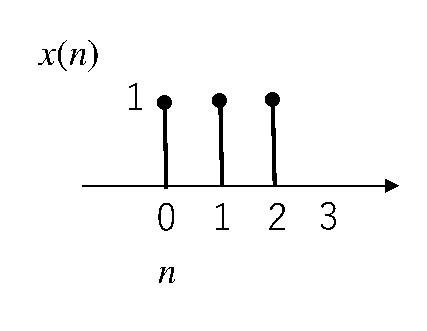
\includegraphics[height=2.6cm]{fig/zu-3e-1b.eps}

(2)
\end{center}
\end{minipage}
\begin{minipage}[b]{.35\textwidth}
\begin{center}
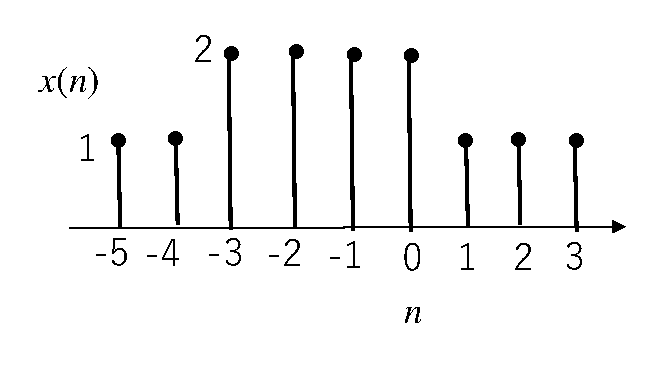
\includegraphics[height=2.5cm]{fig/zu-3e-1c.eps}

(3)
\end{center}
\end{minipage}

\end{center}
%\caption{問題\ref{chapter:3}.1の解図}
\end{figure}



\subsubsection*{問題\ref{chapter:3}.2}
\vskip-\baselineskip
\begin{displaymath}
T_s=\displaystyle \frac{1}{F_s}=2.27 \times 10^{-5}\textrm{sec} \nonumber
\end{displaymath}

このサンプリング周波数である44.1kHzはオーディオにおいて広く用いられるものである.

\subsubsection*{問題\ref{chapter:3}.3}

実際に取り扱うアナログ信号には雑音をはじめとした周波数帯の異なる成分が多く含まれることから,処理のために必要な成分を抽出するために,アナログフィルタを用いる.

\subsection*{第\ref{chapter:ch-2}章}

\subsubsection*{問題\ref{chapter:ch-2}.1}

\begin{enumerate}[(1)]
\item 線形性を満たさない.時普遍性を満たす.

\item 線形性を満たす.時普遍性を満たさない.

\item 線形性を満たす.時普遍性を満たさない.
\end{enumerate}

\subsubsection*{問題\ref{chapter:ch-2}.2}


以下に示す解図のようになる.

\begin{figure}[H]
\begin{center}

\begin{minipage}[b]{.3\textwidth}
\begin{center}
\includegraphics[width=.98\textwidth]{fig/zu-3e-2b.eps}

(1)
\end{center}
\end{minipage}
\begin{minipage}[b]{.3\textwidth}
\begin{center}
\includegraphics[width=.98\textwidth]{fig/zu-3e-2a.eps}

(2)
\end{center}
\end{minipage}
\begin{minipage}[b]{.3\textwidth}
\begin{center}
\includegraphics[width=.98\textwidth]{fig/zu-3e-2c.eps}

(3)
\end{center}
\end{minipage}

\end{center}
%\caption{問題\ref{chapter:ch-2}.2の解図}
\end{figure}

%問題\ref{chapter:ch-2}.3


%以下に示す解図のようになる.

%\begin{figure}[h]
%\begin{center}

%\begin{minipage}{4.5cm}
%\begin{center}
%\includegraphics[width=4.5cm]{fig/zu-3e-3a.eps}

%(1)のハードウェア構成図
%\end{center}
%\end{minipage}
%\begin{minipage}{4.5cm}
%\begin{center}
%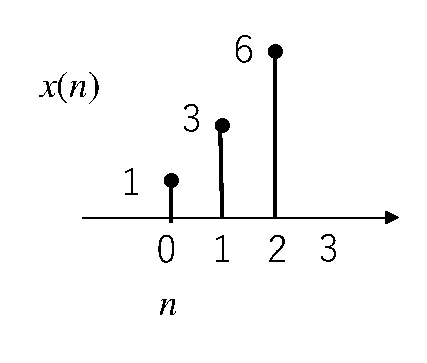
\includegraphics[width=3.5cm]{fig/zu-3e-3b.eps}

%(1)のインパルス応答
%\end{center}
%\end{minipage}

%\begin{minipage}{4.5cm}
%\begin{center}
%\includegraphics[width=4.5cm]{fig/zu-3e-2c.eps}

%(2)のハードウェア構成図
%\end{center}
%\end{minipage}
%\begin{minipage}{4.5cm}
%\begin{center}
%\includegraphics[width=4.5cm]{fig/zu-3e-2c.eps}

%(2)のインパルス応答
%\end{center}
%\end{minipage}

%\end{center}
%\caption{問題\ref{chapter:ch-2}.3の解図}
%\end{figure}


\subsection*{第\ref{chapter:40}章}

\subsubsection*{問題\ref{chapter:40}.1}
\vskip-\baselineskip
\begin{displaymath}
(1)  \hspace{3mm} X(z)=z^2+3-2z^{-1} 
\end{displaymath}
\begin{displaymath}
(2)  \hspace{3mm} X(z) = \frac{1}{1-z^{-1}} + \frac{2z^{-1}}{1-z^{-1}} = \frac{1+2z^{-1}}{1-z^{-1}} 
\end{displaymath}
\begin{displaymath}
(3) \hspace{3mm} X(z)= -b^{-1}z-b^{-2}z^2-b^{-3}z^3- \cdots =\frac{-b^{-1}z}{1-b^{-1}z} = \frac{1}{1-bz^{-1}} \nonumber
\end{displaymath}
\begin{displaymath}
(4) \hspace{3mm} x(n)= \frac{e^{j\omega n}-e^{-j\omega n}}{2j}u(n) \nonumber
\end{displaymath}
と書き換えることができるので\vskip.2\baselineskip
\begin{eqnarray}
X(z)&=&\frac{1}{2j(1-e^{j\omega}z^{-1})} - \frac{1}{2j(1-e^{-j\omega}z^{-1})}=\frac{(1-e^{-j\omega}z^{-1})-(1-e^{j\omega}z^{-1})}{2j(1-e^{-j\omega}z^{-1})(1-e^{j\omega}z^{-1})} \nonumber \\
&=&\frac{e^{j\omega}z^{-1}-e^{-j\omega}z^{-1}}{2j(1-(e^{j\omega}z^{-1}+e^{-j\omega}z^{-1})+z^{-2})}=\frac{\sin (\omega )z^{-1}}{1-2\cos (\omega )z^{-1}+z^{-2}} \nonumber 
\end{eqnarray}
\vskip.5\baselineskip
\subsubsection*{問題\ref{chapter:40}.2}
\vskip-\baselineskip
\begin{displaymath}
(1) \hspace{3mm} Y(z) =aX(z)+bX(z)z^{-d} \nonumber
\end{displaymath}
\begin{displaymath}
(2) \hspace{3mm} Y(z) = \sum_{n=-\infty }^{\infty }(-1)^nx(n)z^{-n} = \sum_{n=-\infty }^{\infty }x(n)(-z)^{-n} =X(-z) \nonumber
\end{displaymath}

\subsection*{第\ref{chapter:42}章}

\subsubsection*{問題\ref{chapter:42}.1}

\noindent (1) べき級数展開法を用いる.
\begin{displaymath}
x(n)=\delta (n+2)+ \delta(n) +2\delta(n-2) \nonumber
\end{displaymath}

\noindent (2) べき級数展開法を用い,$X(z)$を等比級数の和の表現とする.
\begin{displaymath}
X(z)=\sum_{n=0}^{\infty}(0.5z^{-1})^n \nonumber
\end{displaymath}
と書けるため
\begin{displaymath}
x(n)=0.5^nu(n) \nonumber
\end{displaymath}

\noindent (3) 部分分数分解法が既に用いられている.
\begin{displaymath}
x(n)=2(0.5)^nu(n-1)+u(n) \nonumber
\end{displaymath}

\noindent (4) 部分分数分解法を用いる.
\begin{displaymath}
X(z)=\frac{-1}{1-0.5z^{-1}}+\frac{2}{1-z^{-1}} \nonumber
\end{displaymath}
と書けるため
\begin{displaymath}
x(n)=-(0.5)^nu(n)+2u(n) \nonumber
\end{displaymath}

\subsubsection*{問題\ref{chapter:42}.2}
\vskip-\baselineskip
\begin{displaymath}
(1) \hspace{3mm} Y(z)=X(z)+aX(z)z^{-1}+bX(z)z^{-2}=(1+az^{-1}+bz^{-2})X(z) \nonumber 
\end{displaymath}
と書けることから,伝達関数$H(z)$は
\begin{displaymath}
H(z)=\frac{Y(z)}{X(z)}=1+az^{-1}+bz^{-2} \nonumber
\end{displaymath}
であるため,ハードウェア構成は下図のようになる.

%\begin{figure}[H]
\begin{center}
\includegraphics[width=6cm]{fig/zu-9e-1a.eps}
\end{center}
%\caption{システムのハードウェア構成}
%\label{fig:f-9e-a1}
%\end{figure}

\begin{displaymath}
(2) \hspace{3mm} Y(z)=X(z)+aX(z)z^{-1}+bY(z)z^{-2}=(1+az^{-1})X(z)+bz^{-2}Y(z) \nonumber 
\end{displaymath}
と書けることから,伝達関数$H(z)$は
\begin{displaymath}
H(z)=\frac{Y(z)}{X(z)}=\frac{1+az^{-1}}{1-bz^{-2}} \nonumber
\end{displaymath}
であるため,ハードウェア構成は下図のようになる.

%\begin{figure}[H]
\begin{center}
\includegraphics[width=.6\textwidth]{fig/zu-9e-1b.eps}
\end{center}
%\caption{システムのハードウェア構成}
%\label{fig:f-9e-a2}
%\end{figure}

\begin{displaymath}
(3) \hspace{3mm} Y(z)=X(z)+aY(z)z^{-1}+bY(z)z^{-2}=X(z)+(az^{-1}+bz^{-2})Y(z) \nonumber
\end{displaymath}
と書けることから,伝達関数$H(z)$は
\begin{displaymath}
H(z)=\frac{Y(z)}{X(z)}=\frac{1}{1-az^{-1}-bz^{-2}} \nonumber
\end{displaymath}
であるため,ハードウェア構成は下図のようになる.

%\begin{figure}[H]
\begin{center}
\includegraphics[width=.5\textwidth]{fig/zu-9e-1c.eps}
\end{center}
%\caption{システムのハードウェア構成}
%\label{fig:f-9e-a3}
%\end{figure}

\subsubsection*{問題\ref{chapter:42}.3}

\noindent (1) まず周波数特性について,$z$として$e^{j\omega }$を代入すると,
\begin{displaymath}
H(e^{j\omega }) = (1+2e^{-j\omega }+e^{-2j\omega }) = 2e^{-j\omega}(1+\cos(\omega)) \nonumber
\end{displaymath}
と書けるので
\begin{displaymath}
A(e^{j\omega }) = 2(1+\cos(\omega)) \nonumber
\end{displaymath}
\begin{displaymath}
\theta(e^{j\omega }) = -\omega \nonumber
\end{displaymath}
である.

この伝達関数は,
\begin{displaymath}
H(z)=1+2z^{-1}+z^{-2}=(1+z^{-1})^2=\frac{(1+z)^2}{z^2} \nonumber
\end{displaymath}
と書けることから,極は0の重根であり,安定なシステムである.

\noindent (2) まず伝達関数は
\begin{displaymath}
H(z)=\displaystyle \frac{1+2z^{-1}}{2+z^{-1}}=\displaystyle \frac{1+2z^{-1}}{z^{-1}(1+2z)} \nonumber
\end{displaymath}

周波数特性について,$z$として$e^{j\omega }$を代入すると,
\begin{displaymath}
H(e^{j\omega }) = \displaystyle \frac{1+2e^{-j\omega }}{e^{-j\omega }(1+2e^{j\omega })} \nonumber
\end{displaymath}
と書けるので
\begin{displaymath}
A(e^{j\omega }) = \frac{\sqrt{(1+2\cos(\omega))^2+(2\sin(\omega))^2}}{|e^{-j\omega }|\sqrt{(1+2\cos(\omega))^2+(2\sin(\omega))^2}}=1 \nonumber
\end{displaymath}
\begin{eqnarray}
\theta(e^{j\omega }) &=& \tan^{-1}\frac{2\sin(\omega)}{1+2\cos(\omega)}-\tan^{-1}\frac{-2\sin(\omega)}{1+2\cos(\omega)}+\omega \nonumber \\
&=& 2\tan^{-1}\frac{2\sin(\omega)}{1+2\cos(\omega)}+\omega \nonumber
\end{eqnarray}
である.

この伝達関数から,極は$1/2$であり,安定なシステムである.


\subsection*{第\ref{chapter:6}章}

\subsubsection*{問題\ref{chapter:6}.1}
\vskip-\baselineskip
\begin{displaymath}
(1) \hspace{3mm} X(\omega ) = \displaystyle \sum_{n=-^\infty }^{\infty }x(nT)e^{-j \omega nT}= \sum_{n=-^\infty }^{\infty }\delta (nT)e^{-j \omega nT} =1 \nonumber
\end{displaymath}

\begin{eqnarray}
(2) \hspace{3mm} X(\omega ) &=& \displaystyle \sum_{n=-^\infty }^{\infty } \left \{ u(nT)-u(nT-NT) \right \} 
= \sum_{n=0}^{N-1}e^{-j \omega nT} = \frac{1-e^{-jm\omega NT}}{1-e^{-j\omega T}} \nonumber \\
 &=& \frac{\sin 2\omega }{\sin \displaystyle \frac{\omega }{2}} 
\exp \left ( \displaystyle -j \frac{\omega T-j(N-1)}{2} \right ) \nonumber
\end{eqnarray}

\subsubsection*{問題\ref{chapter:6}.2}

\begin{displaymath}
\textrm{(a)} \hspace{3mm} X(j\omega ) = \left ( \displaystyle \frac{\sin \displaystyle \frac{2\omega t}{3}}{\sin \displaystyle \frac{\omega t}{3}} \right ) ^2
\end{displaymath}

\begin{displaymath}
\textrm{(b)} \hspace{3mm} X(j\omega ) = \left ( \displaystyle \frac{\sin \displaystyle \frac{2\omega t}{3}}{\sin \displaystyle \frac{\omega t}{3}} \right ) ^2 e^{-j2\omega t}
\end{displaymath}

\begin{eqnarray}
\textrm{(c)} \hspace{3mm} X(j\omega ) = \left ( \displaystyle \frac{\sin 3\omega t}{\sin \omega t} \right ) ^2 e^{-j4\omega t} \nonumber
\end{eqnarray}

\subsubsection*{問題\ref{chapter:6}.3}

$f_s>3$kHz


\subsection*{第\ref{chapter:a-filter}章}

\subsubsection*{問題\ref{chapter:a-filter}.1}

$-6$dB (常用対数表から$\log_{10}2 \fallingdotseq 0.301$なので$\log_{10}2$を0.3とみなしている)

\subsubsection*{問題\ref{chapter:a-filter}.2}

$C=\displaystyle \frac{1}{2\pi f R} \fallingdotseq 1.6 \times 10^{-6}$Fとなるので1.6$\mu$Fである.

\subsubsection*{問題\ref{chapter:a-filter}.3}

$C=\displaystyle \frac{1}{4\pi^2 f^2 L} \fallingdotseq 2.53 \times 10^{-12}$Fとなるので2.53pFである.


\subsubsection*{問題\ref{chapter:a-filter}.4}\vskip-.2\baselineskip
\begin{displaymath}
I=\displaystyle \left( \frac{V}{R}+ \frac{R}{j\omega L} +j\omega C \right )V \nonumber
\end{displaymath}


\subsection*{第\ref{chapter:dft}章}

\subsubsection*{問題\ref{chapter:dft}.1}

\begin{eqnarray}
\left( 
\begin{array}{cccc}
W^0 & W^0 & W^0 & W^0 \\
W^1 & W^2 & W^3 & W^4 \\
W^2 & W^4 & W^6 & W^8 \\
W^3 & W^6 & W^9 & W^12
\end{array}
\right)
\left( 
\begin{array}{c}
x[0] \\
x[1] \\
x[2] \\
x[3]
\end{array}
\right) = 
\left( 
\begin{array}{cccc}
1 & 1 & 1 & 1 \\
W^1 & W^2 & W^3 & W^4 \\
W^2 & W^4 & W^6 & W^8 \\
W^3 & W^6 & W^9 & W^{12}
\end{array}
\right)
\left( 
\begin{array}{c}
1 \\
1 \\
0 \\
1
\end{array}
\right) = 
\left( 
\begin{array}{c}
3 \\
1 \\
-1 \\
1
\end{array}
\right) \nonumber
\end{eqnarray}

\subsubsection*{問題\ref{chapter:dft}.2}

\begin{eqnarray}
X(k)=\left \{ 
\begin{array}{cc}
-jN/2 & (k=3) \\
jN/2 & (k=N-3) \\
0 & (それ以外)
\end{array}
\right . \nonumber
\end{eqnarray}


\subsection*{第\ref{chapter:fft}章}

\subsubsection*{問題\ref{chapter:fft}.1}

下図のようになる.

%\begin{figure}[H]
\begin{center}
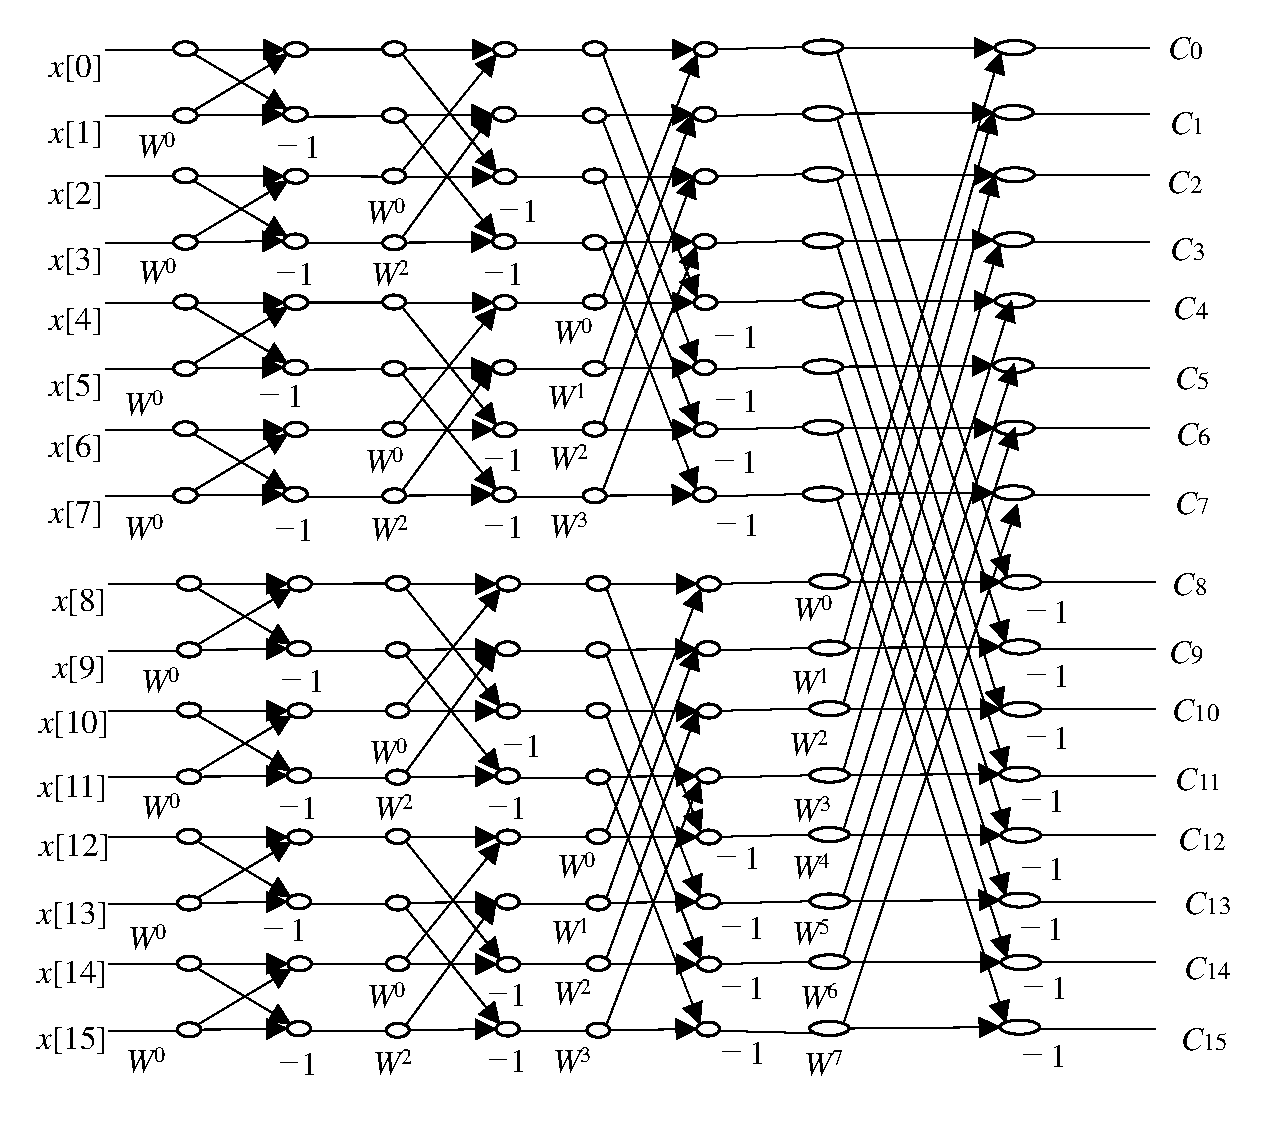
\includegraphics[width=.5\textwidth]{fig/zu-11e-1.eps}
\end{center}
%\caption{問題\ref{chapter:fft}.1の解図}
%\label{fig:zu-12e-01}
%\end{figure}


\subsection*{第\ref{chapter:window}章}

\subsubsection*{問題\ref{chapter:window}.1}

下図(b),(c)を得る.窓長が短いと,メインローブが近接スペクトルを含んでしまい,スペクトルの分離ができないことがわかる.また,サイドローブが大きいと,小さな値のスペクトルを検知することができない.

%\begin{figure}[H]
\begin{center}
\begin{minipage}{.35\textwidth}
\begin{center}
%\includegraphics[width=8cm]{fig/fig-5-14.eps}
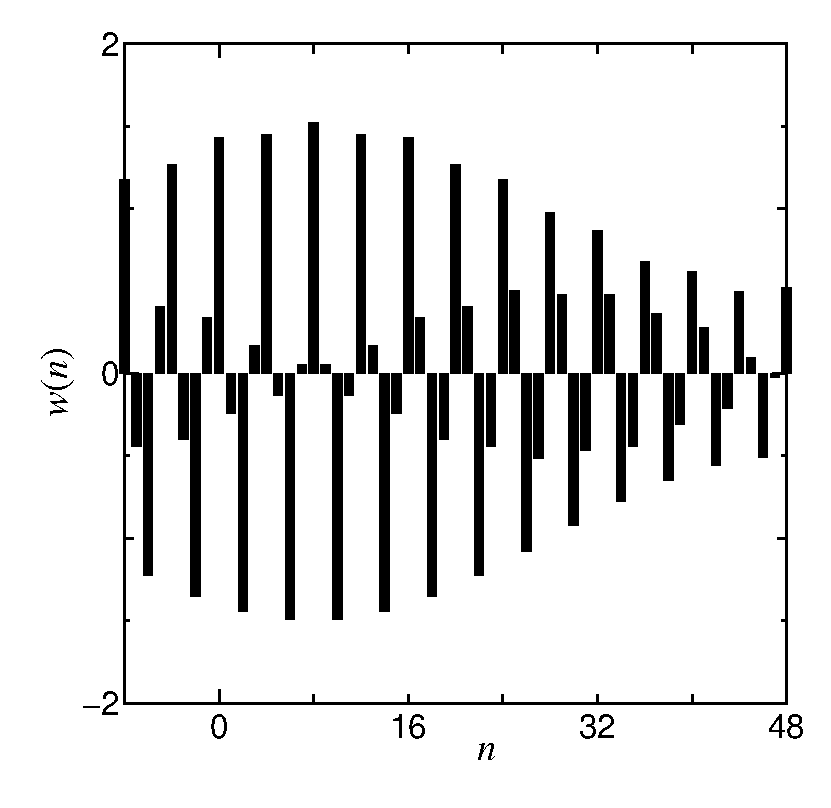
\includegraphics[width=.98\textwidth]{fig/zu-5-14-a.eps}

(a) 信号波形
\end{center}
\end{minipage}
\begin{minipage}{.35\textwidth}
\begin{center}
%\includegraphics[width=8cm]{fig/fig-5-14.eps}
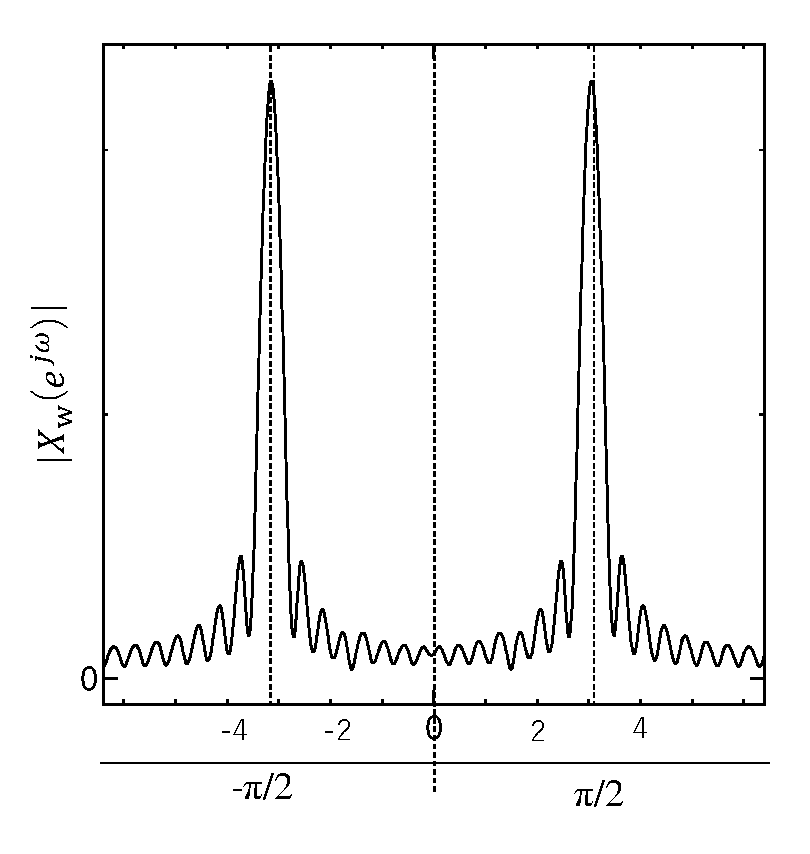
\includegraphics[width=.98\textwidth]{fig/zu-5-14-b.eps}

(b) $M=32$のときのスペクトル
\end{center}
\end{minipage}\\[.5\baselineskip]
\begin{minipage}{.35\textwidth}
\begin{center}
%\includegraphics[width=8cm]{fig/fig-5-14.eps}
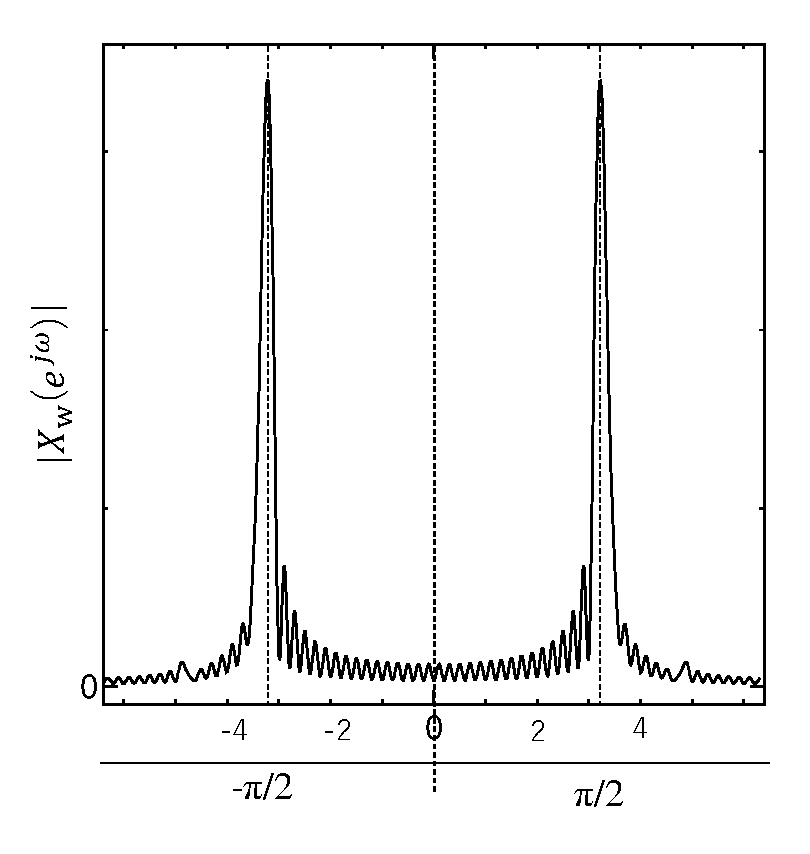
\includegraphics[width=.98\textwidth]{fig/zu-5-14-c.eps}

(c)  $M=64$のときのスペクトル
\end{center}
\end{minipage}
\end{center}
%\caption{例題5.4}
%\label{fig:5-14}
%\end{figure}


\subsection*{第\ref{chapter:11}章}

\subsubsection*{問題\ref{chapter:11}.1}

下図のようになる.

%\begin{figure}[H]
\begin{center}
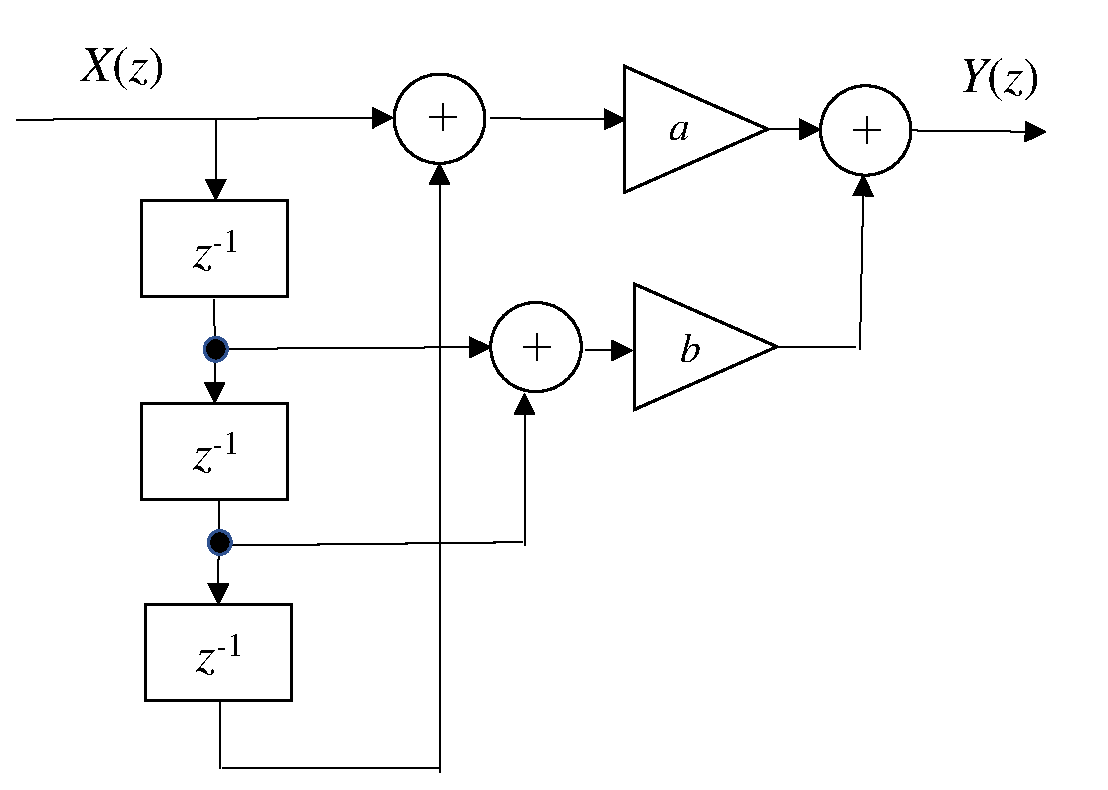
\includegraphics[width=.6\textwidth]{fig/zu-12e-1.eps}
\end{center}
%\caption{問題\ref{chapter:11}.1の解図}
%\label{fig:zu-12e-1}
%\end{figure}



\subsection*{第\ref{chapter:image}章}

\subsubsection*{問題\ref{chapter:image}.1}

下図のようになる.
%\begin{figure}[h]
\begin{center}
\begin{minipage}{7cm}
\begin{center}
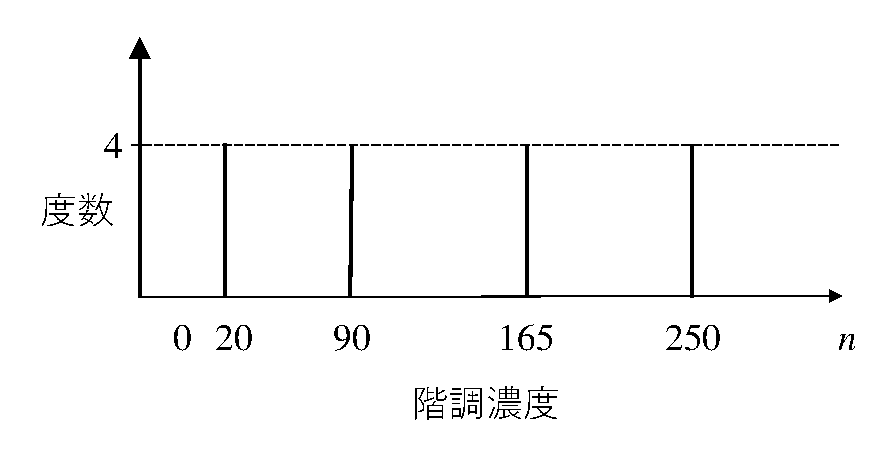
\includegraphics[width=6.5cm]{fig/image_hist.eps}

(1) ヒストグラム
\end{center}
\end{minipage}\\[.5\baselineskip]
\begin{minipage}{.3\textwidth}
\begin{center}
\begin{tabular}{|c|c|c|c|}
\hline
235 & 165 & 90 & 5 \\
\hline 
235 & 165 & 90 & 5 \\
\hline
235 & 165 & 90 & 5 \\
\hline
235 & 165 & 90 & 5 \\
\hline 
\end{tabular}

(2)ネガポジ画像
\end{center}
\end{minipage}\\[.5\baselineskip]
\begin{minipage}[t]{.3\textwidth}
\begin{center}
\begin{tabular}{|c|c|c|c|}
\hline
255 & 0 & 255 & 255 \\
\hline 
0 & 255 & 0 & 255 \\
\hline
0 & 0 & 255 & 255 \\
\hline
0 & 0 & 0 & 255 \\
\hline 
\end{tabular}

(3) ディザ法による2値画像
\end{center}
\end{minipage}\ \ 
\begin{minipage}[t]{.5\textwidth}
\begin{center}
\begin{tabular}{|c|c|c|c|}
\hline
%0 & 8 & 2 & 10 \\
8 & 136 & 40 & 168 \\
\hline 
200 & 72 & 232 & 104 \\
\hline
56 & 184 & 24 & 152 \\
\hline
248 & 120 & 216 & 88 \\
\hline 
\end{tabular}

(3') ディザ法における閾値(図\ref{fig:dither_m}の値に16を掛けて8を足している)
\end{center}
\end{minipage}

%\caption{問題\ref{chapter:image}.1の解図}
%\label{fig:zu-13-1a}
\end{center}
%\end{figure}





\clearpage


\begin{thebibliography}{99}

%ここでは,本書を執筆する上で参考にしたテキストを列挙する.

	\bibitem{電子1} 樋口龍雄,川又政征:``ディジタル信号処理'',昭晃堂(2000)
	\bibitem{電子2} 前田肇:``信号システム理論の基礎'',コロナ社(1997)
	\bibitem{電子3} 貴家仁志:``ディジタル信号処理'',オーム社(2014)
	\bibitem{電子4} 金城繁徳,尾知博:``例題で学ぶディジタル信号処理'',コロナ社(1997)
%	\bibitem{電子5} 井上高宏,常田明夫,江口啓:``例題で学ぶアナログ電子回路'',森北出版(2009)
%	\bibitem{電子6} 尾崎弘,金田彌吉,谷口慶治,横山正人:``電子回路 アナログ編(新訂版)'',共立出版(1989)
%	\bibitem{電子7} 藤井信生:``アナログ電子回路の基礎'',昭晃堂(2004)
	%\bibitem{電子15} 田中賢一:``マンガでわかる電子回路'',オーム社(2009)
\end{thebibliography}

\backmatter
\chapter{謝辞}

本書をまとめるにあたり,近代科学社デジタルファースト編集部の石井沙知編集長をはじめ近代科学社のみなさまに心から感謝申し上げます.

\chapter{著者紹介}

\section*{田中賢一}

1969年7月 宮崎県生まれ

1990年3月 国立都城工業高等専門学校電気工学科卒業

1992年3月 九州工業大学工学部電気工学科卒業

1994年3月 九州工業大学大学院工学研究科博士前期課程修了

九州工業大学工学部助手などを経て,

現在,長崎総合科学大学共通教育部門教授

博士(工学)(九州工業大学)

電子情報通信学会,映像情報メディア学会,画像電子学会,各会員

IEEE Senior Member

画像処理,ホログラフィ,機械学習,教育工学などの研究に従事

%\makelines{10}
%\section{さいごにひと言}
%\makelines{10}
%\subsection{さいごにもうひと言}
%\makelines{100}

%\chapter*{直打ちおわりに}
%\markboth{直打ちおわりに}{直打ちおわりに}
%\addcontentsline{toc}{extchapter}{直打ちおわりに}
%\makelines{10}
%\section*{直打ちさいごにひと言}
%\markright{直打ちさいごにひと言}
%\makelines{10}
%\subsection*{直打ちさいごにもうひと言}
%\makelines{100}

\appendix%%<- 後付け付録を許容しました。
%\begin{lead}
%ここでは、大学1回生で習う微分積分学の基本定理から始まり、
%中心極限定理の証明まで復習します。
%\end{lead}
%\chapter{付録:微分積分学の基本}
%ここでは、大学1回生で習う微分積分学の基本定理から始まり、
%中心極限定理の証明まで復習します。
%\section{微分積分学の基本定理}
%\makelines{10}
%\section{中間値の定理}
%\makelines{100}

%\begin{lead}
%ここでは、大学1回生で習うベクトル空間から始まり、
%スペクトル分解まで復習します。
%\end{lead}
%\chapter{数学的な補足}
%ここでは、大学1回生で習うベクトル空間から始まり、
%スペクトル分解まで復習します。
%\section{ベクトル空間}
%\makelines{10}
%\section{線型写像}
%\makelines{10}
%\section{スペクトル分解}
%\makelines{100}

\printindex
\end{document}
